%
\documentclass[11pt]{article}
\newcommand{\teilnr}{III}
\usepackage{xr}
\externaldocument{../teil1/main_teil1}
\externaldocument{../teil2/main_teil2}
%
%
\usepackage[margin=1.2in]{geometry}
\usepackage{graphicx}
%
\makeatletter\newcommand*{\captionfigur}{\def\@captype{figure}\caption}\makeatother
\usepackage{tikz}\usetikzlibrary{fit,calc,arrows.meta,backgrounds}   %
%
\renewcommand{\topfraction}{0.85}\renewcommand{\textfraction}{0.1}\renewcommand{\floatpagefraction}{0.75}
\graphicspath{{../abbildungen/}}   %
\usepackage[T1]{fontenc}
\usepackage{lmodern}
\usepackage{amsmath,amssymb,amsthm}
\usepackage{etoolbox}
\usepackage{refcount}
\usepackage{array}       %
\usepackage{longtable}   %
\usepackage[hidelinks]{hyperref}

\providecommand{\teilnr}{?}
\newif\ifimband

%
\newtheorem{theorem}{Theorem}[section]
\newtheorem{proposition}[theorem]{Proposition}
\newtheorem{lemma}[theorem]{Lemma}
\newtheorem{corollary}[theorem]{Corollary}
\theoremstyle{definition}
\newtheorem{definition}[theorem]{Definition}
\theoremstyle{remark}
\newtheorem{remark}[theorem]{Remark}
\newtheorem{question}[theorem]{Question}
\renewcommand{\thetheorem}{\teilnr.\arabic{section}.\arabic{theorem}}
\numberwithin{equation}{section}
%
%
\def\theHtheorem{\teilnr.\arabic{section}.\arabic{theorem}}
\def\theHsection{\teilnr.\arabic{section}}
\def\theHequation{\teilnr.\arabic{section}.\arabic{equation}}

%
%
%
%
\newcommand{\tlabel}[1]{\label{\teilnr:#1}}
%
%
%
\newwrite\belegaus
\immediate\openout\belegaus=\jobname.bel
\newcommand{\belegart}[1]{\immediate\write\belegaus{\thetheorem|#1|\thesection}{\normalfont\small[#1]}\ }
\newcommand{\tref}[1]{\ref{\teilnr:#1}}
\makeatletter
\newcommand{\partref}[2]{%
  \edef\serie@teil{\teilnr}\def\serie@ziel{#1}%
  \ifx\serie@teil\serie@ziel\ref{#1:#2}%
  \else\ifimband\ref{#1:#2}%
  \else\getrefnumber{#1:#2}~in~[Part~#1]\fi\fi}
\makeatother

%
%
%
%
\makeatletter
%
\@namedef{Z@nenner}{811}
%
\@namedef{Z@offen}{6}
%
\@namedef{Z@erledigt}{805}
%
\@namedef{Z@zertifiziert}{767}
%
\@namedef{Z@vollzerlegt}{38}
%
\@namedef{Z@csechsquadrat}{1.3685}
%
\@namedef{Z@csechswalker}{0.3137}
%
\@namedef{Z@csechs}{1.6822}
%
\@namedef{Z@streifenfam}{206}
%
\@namedef{Z@streifentot}{52}
%
\@namedef{Z@streifentuerme}{154}
%
\@namedef{Z@streifenstellen}{8.4\cdot 10^{7}}
%
\@namedef{Z@streifenminm}{223}
%
\@namedef{Z@streifensieben}{17.5}
%
\@namedef{Z@streifeneins}{2}
%
\@namedef{Z@margestich}{530}
%
\@namedef{Z@margemax}{10^{8}}
%
\@namedef{Z@margerand}{2\cdot 10^{5}}
%
\@namedef{Z@margemin}{21.5}
%
\@namedef{Z@streifenschranke}{2000}
%
\@namedef{Z@streifensteckt}{14}
%
\@namedef{Z@glattkerne}{889\,437}
%
\@namedef{Z@glattkand}{0}
%
\@namedef{Z@glattunten}{10^{8}}
%
\@namedef{Z@glattoben}{10^{15}}
%
\@namedef{Z@glatthoehe}{2000}
%
\@namedef{Z@glattprim}{100}
%
\@namedef{Z@glattmin}{4}
%
\@namedef{Z@glattperiode}{9573}
%
\@namedef{Z@glattgross}{356\,888}
%
\@namedef{Z@glattrest}{532\,549}
%
\@namedef{Z@bboxkern}{10^{6}}
%
\@namedef{Z@bboxb}{10^{4}}
%
\@namedef{Z@bboxfam}{101\,329}
%
\@namedef{Z@bboxparitaet}{32\,118}
%
\@namedef{Z@bboxpaare}{421\,010\,513}
%
\@namedef{Z@bboxohnealpha}{343\,504\,538}
%
\@namedef{Z@bboxzweiadisch}{16\,603\,302}
%
\@namedef{Z@bboxkgerade}{11\,242\,224}
%
\@namedef{Z@bboxlemmal}{49\,659\,524}
%
\@namedef{Z@bboxrest}{925}
%
\@namedef{Z@ballotfaelle}{56}
%
\@namedef{Z@ballotgedruckt}{0}
%
\@namedef{Z@ballotfib}{50}
%
\@namedef{Z@turmk1}{1.1\cdot 10^{13}}
%
\@namedef{Z@turmk2}{5.5\cdot 10^{13}}
%
\@namedef{Z@turmk3}{4.5\cdot 10^{30}}
%
\@namedef{Z@turmstellen}{2.5\cdot 10^{15}}
%
\@namedef{Z@kongruenzbis}{10^{5}}
%
\@namedef{Z@kongruenzdichte}{2.67\cdot 10^{-4}}
%
\@namedef{Z@yokoimax}{20000}
%
\@namedef{Z@yokoipaare}{123}
%
\@namedef{Z@designkerne}{251}
%
\@namedef{Z@designtmax}{399}
%
\@namedef{Z@designfenster}{17}
%
\@namedef{Z@designmaxm}{1023}
%
\@namedef{Z@designstellen}{2000}
%
\@namedef{Z@quadratzeuge1}{701}
%
\@namedef{Z@quadratzeuge2}{3}
%
\@namedef{Z@quadratzeuge3}{5}
%
\@namedef{Z@mittenquadrat}{0.3648}
%
\@namedef{Z@mittendoppel}{0.2580}
%
\@namedef{Z@mittensatza}{0.6228}
%
\@namedef{Z@mittenN}{10^{14}}
%
\@namedef{Z@mittengemessen}{0.6252}
%
\@namedef{Z@kerne}{10\,132\,126}
%
\@namedef{Z@kernschranke}{10^{8}}
%
\@namedef{Z@hoehe}{2000}
%
\@namedef{Z@zeugenschranke}{2\cdot 10^{5}}
%
\@namedef{Z@filterfamilien}{83}
%
\@namedef{Z@punktfamilien}{79}
%
\@namedef{Z@punkte}{445}
%
\@namedef{Z@paritaetspunkte}{74}
%
\@namedef{Z@zeugenpunkte}{371}
%
\@namedef{Z@restpunkte}{0}
%
\@namedef{Z@beispielm}{7}
%
\@namedef{Z@beispielk}{7}
%
\@namedef{Z@beispielzeuge}{29}
%
\@namedef{Z@beispielwert}{130\,576\,328}
%
\@namedef{Z@beispielfaktoren}{2^{3}\cdot 29\cdot 197\cdot 2857}
%
\@namedef{Z@ohnetripel}{3.88\cdot 10^{20}}
%
\@namedef{Z@ohnetripelsicher}{1.83\cdot 10^{18}}
%
\@namedef{Z@famtab}{(2, 1) & 1 & 0.90 & 1.53 & 14 \\
(3, 1) & 3 & 2.83 & 3.43 & 6 \\
(23, 2) & 1 & 4.09 & 9.37 & 2 \\
(6, 1) & 3 & 5.37 & 5.97 & 3 \\
(1, 5) & 5 & 5.67 & 12.54 & 2 \\
(46, 1) & 1 & 8.77 & 9.37 & 2 \\
(7, 2) & 7 & 9.73 & 20.67 & 1 \\
(5, 1) & 5 & 11.94 & 12.54 & 1 \\
(430, 1) & 1 & 12.91 & 13.52 & 1 \\
(79, 23) & 1 & 13.08 & 27.36 & 1 \\
(3, 7) & 7 & 13.69 & 28.58 & 1 \\
(10, 1) & 5 & 15.19 & 15.79 & 1 \\
(7, 1) & 7 & 16.23 & 16.83 & 1 \\
(14, 1) & 7 & 20.07 & 20.67 & 1 \\
(1022, 57) & 1 & 20.21 & 41.62 & 1 \\
(19, 35) & 5 & 21.59 & 44.38 & 1 \\}
%
\@namedef{Z@famzahl}{16}
%
\@namedef{Z@famtabzwei}{14}
%
\@namedef{Z@fampaare}{39}
%
\@namedef{Z@famquadrat}{32}
%
\@namedef{Z@famohne}{7}
%
\@namedef{Z@paargrenze}{3.89\cdot 10^{21}}
%
\@namedef{Z@paarletzt}{3\,887\,785\,221\,910\,670\,811\,499}
%
\@namedef{Z@periodepk}{6082}
%
\@namedef{Z@periodepkmax}{10\,000}
%
\@namedef{Z@walkerpk}{955}
%
\@namedef{Z@walkerpkmax}{3000}
%
\@namedef{Z@paare52}{26}
%
\@namedef{Z@paare52exp}{52}
%
\@namedef{Z@mersennemax}{63}
%
\@namedef{Z@famquadratfam}{10}
%
\@namedef{Z@quadratbmax}{10^{4}}
%
\@namedef{Z@walkerdmax}{10^{6}}
%
\@namedef{Z@expfam}{750}
%
\@namedef{Z@expmmax}{10^{4}}
%
\@namedef{Z@exppmax}{3000}
%
\@namedef{Z@exppaare}{120\,373}
%
\@namedef{Z@expwzwei}{470}
%
\@namedef{Z@expwdrei}{52}
%
\@namedef{Z@exphzwei}{486}
%
\@namedef{Z@exphdrei}{49.1}
%
\@namedef{Z@korrs}{411.7}
%
\@namedef{Z@korrmu}{436.2}
%
\@namedef{Z@korrsd}{28.2}
%
\@namedef{Z@korrreps}{4000}
%
\@namedef{Z@korrz}{-0.87}
%
\@namedef{Z@korrp}{0.80}
%
\@namedef{Z@korrvert}{396, 255, 83, 15, 1}
%
\@namedef{Z@korrmaxp}{181}
%
\@namedef{Z@korrmaxz}{2.4}
%
\@namedef{Z@trennvoll}{652}
%
\@namedef{Z@trennzwei}{90}
%
\@namedef{Z@trennfuenf}{48}
%
\@namedef{Z@trennlaeufe}{40}
%
\@namedef{Z@alekterme}{33}
%
\@namedef{Z@alekstellen}{67}
%
\@namedef{Z@klassedreimax}{10^{8}}
%
\@namedef{Z@alekneun}{9}
%
\@namedef{Z@vollexpo}{36}
%
\@namedef{Z@vollmexpo}{24}
%
\@namedef{Z@reinhartt1}{94}
%
\@namedef{Z@reinharttab}{4\,099\,215 & 228 & $2\cdot 10^{5}$ & 701, 100469, 157049 & $1.1\cdot 10^{13}$ & $2.5\cdot 10^{15}$ \\
39\,028\,039\,587\,479 & 1\,880\,030 & $3\cdot 10^{3}$ & 5, 7, 71, 1657; 19, 29, 421, 569, 1987; 379, 2089, 2203, 2437 & $4.5\cdot 10^{30}$ & $8.6\cdot 10^{36}$ \\}
%
\@namedef{Z@reinhartungerade}{209\,991}
%
\@namedef{Z@reinhartungerade2}{117\,477\,414\,815}
%
\@namedef{Z@reinhartboxk}{1, 3, 5, 7}
%
\@namedef{Z@reinhartboxz}{701, 11, 19, 29}
%
\@namedef{Z@reinhartungeradest}{95}
%
\@namedef{Z@reinhartungeradest2}{11\,621}
%
\@namedef{Z@zeugenalle}{371}
%
\@namedef{Z@zeugenprim}{8}
%
\@namedef{Z@zeugenmedian}{19}
%
\@namedef{Z@zeugenmax}{114\,997}
%
\@namedef{Z@zeugen29}{79}
%
\@namedef{Z@zeugen19}{78}
%
\@namedef{Z@zeugen11}{45}
%
\@namedef{Z@zeugen3}{43}
%
\@namedef{Z@zeugen5}{33}
%
\@namedef{Z@zeugen7}{25}
%
\@namedef{Z@zeugennkp}{197}
%
\@namedef{Z@zeugennkk}{1379}
%
\@namedef{Z@zeugennkv}{2}
%
\@namedef{Z@rizzierfuellt}{328}
%
\@namedef{Z@rizzinicht}{43}
%
\@namedef{Z@kongrp}{10^{6}}
%
\@namedef{Z@kongrkerne}{15}
%
\@namedef{Z@kongrpaare}{425\,362}
%
\@namedef{Z@bedpunkte}{445}
%
\@namedef{Z@bedteiler}{2149}
%
\@namedef{Z@bedausweg}{1682}
%
\@namedef{Z@bedanteil}{78.3}
%
\@namedef{Z@bedmedian}{3}
%
\@namedef{Z@bedmittel}{3.8}
%
\@namedef{Z@bedmax}{12}
%
\@namedef{Z@bedallemedian}{4}
%
\@namedef{Z@bedallemax}{16}
%
\@namedef{Z@besp}{3\cdot 10^{6}}
%
\@namedef{Z@beskerne}{25}
%
\@namedef{Z@besnp}{5}
%
\@namedef{Z@bespunkte}{378}
%
\@namedef{Z@besraenge}{2536}
%
\@namedef{Z@besbesetzt}{2025}
%
\@namedef{Z@beszeuge}{1988}
%
\@namedef{Z@beszeugeant}{98.17}
%
\@namedef{Z@beswief}{37}
%
\@namedef{Z@besleer}{511}
%
\@namedef{Z@beseinsnp}{1}
%
\@namedef{Z@beseinszeuge}{1936}
%
\@namedef{Z@beseinsant}{95.60}
%
\@namedef{Z@beseinswief}{89}
%
\@namedef{Z@rgpaare}{961}
%
\@namedef{Z@rgkerne}{79}
%
\@namedef{Z@rgerledigt}{954}
%
\@namedef{Z@rgzert}{954}
%
\@namedef{Z@rgvoll}{0}
%
\@namedef{Z@pbbausteine}{41}
%
\@namedef{Z@pbzahlen}{24}
%
\@namedef{Z@pbpock}{18}
%
\@namedef{Z@pbecpp}{6}
%
\@namedef{Z@pbpockmax}{75}
%
\@namedef{Z@pbecppmax}{477}
%
\@namedef{Z@rgoffen}{7}
%
\@namedef{Z@rgprpzeuge}{0}
%
\@namedef{Z@rgbedingt}{0}
%
\@namedef{Z@teilevollm}{23}
%
\@namedef{Z@teilevolld}{161}
%
\@namedef{Z@teilevolla}{111}
%
\@namedef{Z@teilevollb}{112}
%
\@namedef{Z@teilezeugem}{7}
%
\@namedef{Z@teilezeuged}{1449}
%
\@namedef{Z@teilezeugest}{477}
%
\@namedef{Z@rgaltkerne}{25}
%
\@namedef{Z@rgneukerne}{54}
%
\@namedef{Z@rgungerade}{21}
%
\@namedef{Z@wegetab}{certified witness: search by position, small primes & 605 & 103 & 708 \\
certified witness: search by position, congruence filter & 64 & 16 & 80 \\
certified witness: elliptic curves and $p - 1$ (SymPy) & 70 & 0 & 70 \\
certified witness: elliptic curves (GMP-ECM) & 27 & 20 & 47 \\
certified witness: $M_d$ itself prime, with a certificate & 8 & 8 & 16 \\
certified witness: complete factorization, factors proved prime & 32 & 0 & 32 \\
certified witness: a factor of the algebraic split, proved prime & 1 & 0 & 1 \\
open & 4 & 3 & 7 \\}
%
\@namedef{Z@bouchardn}{9800}
%
\@namedef{Z@bouchardp}{13}
%
\@namedef{Z@bouchardfakt}{2\cdot 13^{2}\cdot 29}
%
\@namedef{Z@pellwief}{13,\ 31,\ 1546463}
%
\@namedef{Z@reinhartza}{701}
%
\@namedef{Z@reinhartzc}{5}
%
\@namedef{Z@offentab}{399 & 171 & 173 & 300 & 1071 & 2753 & 8.36 & 1.10 \\
407 & 111 & 269 & 300 & 1071 & 2753 & 8.36 & 1.10 \\
39 & 247 & 367 & 300 & 1071 & 2753 & 8.36 & 1.10 \\
111 & 185 & 400 & 300 & 1071 & 2753 & 8.36 & 1.10 \\
407 & 259 & 805 & 300 & 1071 & 2753 & 8.05 & 1.05 \\
663 & 663 & 889 & 300 & 1071 & 38 & 1.05 & 0.11 \\
20\,303 & 257 & 1893 & 300 & 209 & -- & 0.22 & 0.02 \\}
%
\@namedef{Z@wfinpop}{3}
%
\@namedef{Z@offenmin}{173}
%
\@namedef{Z@erstesucheP}{3\cdot 10^{6}}
%
\@namedef{Z@siebober}{10^{9}}
%
\@namedef{Z@prtripel}{1341}
%
\@namedef{Z@prvauf1}{1338}
%
\@namedef{Z@prvauf2}{3}
%
\@namedef{Z@prerwartet}{2.38}
%
\@namedef{Z@zweip}{10^{6}}
%
\@namedef{Z@zweiamax}{100\,000}
%
\@namedef{Z@zweiexp}{99\,999}
%
\@namedef{Z@zweiminus}{8957}
%
\@namedef{Z@zweiminusant}{8.96}
%
\@namedef{Z@zweiplus}{2511}
%
\@namedef{Z@zweiplusant}{2.51}
%
\@namedef{Z@zweiminusok}{91\,042}
%
\@namedef{Z@zweiplusok}{97\,488}
%
\@namedef{Z@zweistellen}{30\,103}
%
\@namedef{Z@wfereignisse}{54}
%
\@namedef{Z@wfprimzahlen}{40}
%
\@namedef{Z@wfkerne}{79}
%
\@namedef{Z@wfp}{3\cdot 10^{6}}
%
\@namedef{Z@wfungerade}{18}
%
\@namedef{Z@wfgerade}{15}
%
\@namedef{Z@wfzeuge}{11}
%
\@namedef{Z@wfoffen}{3}
%
\@namedef{Z@wfentschieden}{12}
%
\@namedef{Z@wfmgross}{1\,375\,502\,561}
%
\@namedef{Z@wfmgroesser}{158\,585\,313\,121}
%
\@namedef{Z@wfmquadrat}{20161}
%
\@namedef{Z@erstesuchekerne}{25}
%
\@namedef{Z@lucasgleich}{16}
%
\@namedef{Z@lucaspk}{3}
%
\@namedef{Z@lucasnk}{25}
%
\@namedef{Z@wftab}{15 & 45 & 181 & witness & yes \\
31 & 39 & 157 & witness & no \\
79 & 253 & 4049 & witness & no \\
143 & 13 & 311 & witness & yes \\
223 & 45 & 179 & witness & no \\
319 & 5 & 20\,161 & complete factorization & yes \\
383 & 21545 & 258\,539 & witness & no \\
447 & 413 & 24\,781 & witness & no \\
455 & 9 & 37 & witness & no \\
615 & 807 & 3229 & not settled & no \\
1343 & 5 & 19 & witness & no \\
1535 & 63 & 251 & witness & no \\
2135 & 13 & 53 & witness & no \\
2135 & 37 & 149 & not settled & no \\
123\,879 & 9 & 37 & not settled & no \\}
%
\@namedef{Z@wfinpopzu}{3}
%
\@namedef{Z@wfnullrang}{16}
%
\@namedef{Z@csechsbmax}{10^{6}}
%
\@namedef{Z@csechsfamq}{676\,094}
%
\@namedef{Z@csechsfamw}{275\,371}
%
\@namedef{Z@kdkerne}{10\,132\,121}
%
\@namedef{Z@kdschranke}{10^{8}}
%
\@namedef{Z@kdkandidaten}{86}
%
\@namedef{Z@kdpunkte}{883}
%
\@namedef{Z@kdungerade}{51}
%
\@namedef{Z@kdpaare}{832}
%
\@namedef{Z@kdkernmax}{3\,926\,299}
%
\@namedef{Z@kdpaarkerne}{57}
%
\@namedef{Z@kddrei}{583}
%
\@namedef{Z@kdreinhartst}{99\,134}
%
\@namedef{Z@kdreinhartungst}{117}
%
\@namedef{Z@turmtab}{100 & 14 & 37 & 21 & 67 \\
250 & 39 & 97 & 53 & 168 \\
500 & 83 & 199 & 111 & 344 \\
1000 & 176 & 410 & 224 & 695 \\
1500 & 270 & 616 & 345 & 1049 \\
2000 & 371 & 832 & 467 & 1404 \\}
%
\@namedef{Z@turmc7}{0.1817}
%
\@namedef{Z@turmc3}{0.4134}
%
\@namedef{Z@turmc}{0.595}
%
\@namedef{Z@turmtuerme}{122}
%
\@namedef{Z@turmtuerme7}{60}
%
\@namedef{Z@turmtuerme3}{62}
%
\@namedef{Z@turmueber}{111.8}
%
\@namedef{Z@wtab}{1 & 0.0594 & 0.2914 \\
2 & 0.1341 & 0.3666 \\
3 & 0.1711 & 0.4027 \\
4 & 0.1936 & 0.4212 \\
5 & 0.2047 & 0.4366 \\
6 & 0.2151 & 0.4513 \\
7 & 0.2217 & 0.4566 \\}
%
\@namedef{Z@modellp}{31}
%
\@namedef{Z@modell7min}{0.94}
%
\@namedef{Z@modell7max}{1.01}
%
\@namedef{Z@modell3min}{0.91}
%
\@namedef{Z@modell3max}{1.04}
%
\@namedef{Z@beins7}{87.1}
%
\@namedef{Z@beins3}{86.3}
%
\@namedef{Z@einkernm}{525\,003}
%
\@namedef{Z@einkernanteil}{45}
%
\@namedef{Z@modellc}{0.7482}
%
\@namedef{Z@modellrate}{0.8835}
%
\@namedef{Z@naivrate}{1.1808}
%
\@namedef{Z@modelltab}{8 & 10 & 11.5 & 15.4 \\
10 & 14 & 15.5 & 20.7 \\
12 & 18 & 19.5 & 26.0 \\
14 & 24 & 23.5 & 31.4 \\
16 & 26 & 27.6 & 36.9 \\
18 & 31 & 31.6 & 42.3 \\
20 & 35 & 35.7 & 47.7 \\}
%
\@namedef{Z@modellnull}{39}
%
\@namedef{Z@modellnullkorr}{38.94}
%
\@namedef{Z@modellnullnaiv}{52.04}
%
\@namedef{Z@modellneu}{13}
%
\@namedef{Z@modellneukorr}{12.06}
%
\@namedef{Z@modellneunaiv}{16.12}
%
\@namedef{Z@quadbmax}{10^{4}}
%
\@namedef{Z@quadtab}{49.7 & 32 & 38.9 & 52.0 & 0.7049 \\
75.0 & 54 & 61.3 & 81.9 & 0.7744 \\
100.0 & 76 & 83.4 & 111.4 & 0.8136 \\
150.0 & 124 & 127.5 & 170.4 & 0.8755 \\
200.0 & 171 & 171.7 & 229.5 & 0.9011 \\
300.0 & 265 & 260.1 & 347.6 & 0.9300 \\
500.0 & 468 & 436.8 & 583.7 & 0.9765 \\
1000.0 & 997 & 878.5 & 1174.1 & 1.0345 \\}
%
\@namedef{Z@quadkreuz}{192.9}
%
\@namedef{Z@quadkreuzlog}{83.8}
%
\@namedef{Z@quadgeboren}{103}
%
\@namedef{Z@quadrate1000}{1.0345}
%
\@namedef{Z@quadnq1000}{997}
%
\@namedef{Z@quadv1000}{878.5}
%
\@namedef{Z@quadrest1000}{894}
%
\@namedef{Z@teilsumq1}{0.6055}
%
\@namedef{Z@teilsumq2}{0.8949}
%
\@namedef{Z@teilsumtab}{3 & 1.1044 & 0.1783 & 1.2827 \\
4 & 1.2235 & 0.2385 & 1.4619 \\
5 & 1.3110 & 0.2831 & 1.5941 \\
6 & 1.3685 & 0.3137 & 1.6822 \\}
%
\@namedef{Z@zuwq}{79}
%
\@namedef{Z@zuww}{77}
%
\@namedef{Z@zuwtopq}{71}
%
\@namedef{Z@zuwtopw}{72}
%
\@namedef{Z@a1nmax}{10^{12}}
%
\@namedef{Z@a1dmax25}{10^{5}}
%
\@namedef{Z@a1paare25}{18}
%
\@namedef{Z@a1dmax}{20\,000}
%
\@namedef{Z@a1kerne}{12\,159}
%
\@namedef{Z@a1paare}{6063}
%
\@namedef{Z@a1hoehe}{2000}
%
\@namedef{Z@a1ueber}{7}
%
\@namedef{Z@a1paareh}{6056}
%
\@namedef{Z@a1p1}{5\cdot 10^{5}}
%
\@namedef{Z@a1zeuge1}{4991}
%
\@namedef{Z@a1p2}{5\cdot 10^{6}}
%
\@namedef{Z@a1zeuge2}{154}
%
\@namedef{Z@a1rest2}{918}
%
\@namedef{Z@a1s2prim}{24}
%
\@namedef{Z@a1s2primzert}{5}
%
\@namedef{Z@a1s2ecm}{15}
%
\@namedef{Z@a1s2offen}{879}
%
\@namedef{Z@a1s2kleinst}{81}
%
\@namedef{Z@a1s2probable}{19}
%
\@namedef{Z@a1s2ecpp}{19}
%
\@namedef{Z@a1s2ecppmax}{1687}
%
\@namedef{Z@a1s2nk}{5}
%
\@namedef{Z@quadzeilen}{8}
%
\@namedef{Z@quadab}{300}
%
\@namedef{Z@quadablog}{130}
%
\@namedef{Z@quadslack}{6}
%
\@namedef{Z@wtabmax}{10^{7}}
%
\@namedef{Z@reinhartgerade}{3}
%
\@namedef{Z@reinhartgeradesicher}{1}
%
\@namedef{Z@reinhartsieben}{4}
%
\@namedef{Z@znab}{300}
%
\@namedef{Z@znaq}{183}
%
\@namedef{Z@znaqg}{182}
%
\@namedef{Z@znamit}{34}
%
\@namedef{Z@phidreilavij}{13}
%
\@namedef{Z@phidreibrute}{10^{6}}
%
\@namedef{Z@phidreistellen}{19, 35 and 52}
%
\@namedef{Z@phidreiperiode}{7}
%
\@namedef{Z@zyktab}{3 & 18 & 343 & $7^{3}$ \\
3 & 88\,916 & 7\,906\,143\,973 & $7^{2}\cdot 13^{3}\cdot 271^{2}$ \\
4 & 682 & 465\,125 & $5^{3}\cdot 61^{2}$ \\
5 & 3 & 121 & $11^{2}$ \\
6 & 19 & 343 & $7^{3}$ \\
6 & 88\,917 & 7\,906\,143\,973 & $7^{2}\cdot 13^{3}\cdot 271^{2}$ \\}
%
\@namedef{Z@zykn}{3\,004\,199}
%
\@namedef{Z@zyktreffer}{6}
%
\@namedef{Z@zykschranke}{10^{12}}
%
\@namedef{Z@zykklasse}{10^{14}}
%
\@namedef{Z@lstab}{$10^{12}$ & 2\,158\,391 & 832\,161 & 0.31 & 900 & 69 & 1656 & 183 of 215 \\
$10^{13}$ & 6\,840\,384 & 2\,593\,517 & 0.18 & 44\,100 & 57 & 63\,900 & 189 of 211 \\
$10^{14}$ & 21\,663\,503 & 8\,235\,300 & 0.10 & 44\,100 & 48 & 63\,900 & 191 of 201 \\}
%
\@namedef{Z@lsnpw}{21\,663\,503}
%
\@namedef{Z@lswerte}{8\,235\,300}
%
\@namedef{Z@lsanteil}{0.10}
%
\@namedef{Z@lsbis}{48}
%
\@namedef{Z@lsocc}{112}
%
\@namedef{Z@lserster}{63\,900}
%
\@namedef{Z@lsg100}{103}
%
\@namedef{Z@lsg100pw}{102}
%
\@namedef{Z@lsg200}{201}
%
\@namedef{Z@lsg200pw}{191}
%
\@namedef{Z@lserwartet}{0.05}
%
\@namedef{Z@lsdecke}{63\,900 & 900 & 9 & 112 & 50.9 \\
82\,908 & 1764 & 36--41 & 98 & 49.0 \\
17\,100 & 900 & 9 & 97 & 43.3 \\
23\,324 & 1372 & 170--175 & 96 & 20.8 \\
151\,900 & 4900 & 10--11 & 90 & 45.6 \\
171\,900 & 900 & 9 & 90 & 52.2 \\
7100 & 100 & 357--381 & 89 & 61.8 \\
26\,100 & 900 & 9 & 89 & 37.1 \\
127\,800 & 1800 & 29--31 & 89 & 53.9 \\
215\,100 & 900 & 9 & 89 & 51.7 \\}
%
\@namedef{Z@lsdeckeanz}{10}
%
\@namedef{Z@lsg20}{21}
%
\@namedef{Z@lsanteilpw}{24.2--44.9}
%
\@namedef{Z@lsanteilnpw}{20.8--61.8}
%
\@namedef{Z@nvlmax}{50}
%
\@namedef{Z@nvrel}{1.2}
%
\@namedef{Z@nvsteig}{0.63}
%
\@namedef{Z@lstop1}{44\,100}
%
\@namedef{Z@zmn}{62\,118}
%
\@namedef{Z@zmmin}{20}
%
\@namedef{Z@lsbasiswerte}{62\,118}
%
\@namedef{Z@lsbasismind}{20}
%
\@namedef{Z@lsbasisanteil}{4.81}
%
\@namedef{Z@lsbasiserw}{2.4}
%
\@namedef{Z@fpn}{3531}
%
\@namedef{Z@fpmax}{3\cdot 10^{-16}}
%
\@namedef{Z@zmr2}{0.545}
%
\@namedef{Z@zmr2sd}{0.025}
%
\@namedef{Z@zmroh}{0.306}
%
\@namedef{Z@zmrohsd}{0.005}
%
\@namedef{Z@zmr2log}{0.514}
%
\@namedef{Z@zmr2logsd}{0.016}
%
\@namedef{Z@zmallesep}{0.319}
%
\@namedef{Z@zmallesepsd}{0.012}
%
\@namedef{Z@zmalleroh}{0.307}
%
\@namedef{Z@zmallerohsd}{0.004}
%
\@namedef{Z@zmdeutstufen}{3061}
%
\@namedef{Z@zmdeutkmin}{4}
%
\@namedef{Z@zmkern}{0.012}
%
\@namedef{Z@zmkof}{0.272}
%
\@namedef{Z@zmww}{0.001}
%
\@namedef{Z@zmkerne}{2986}
%
\@namedef{Z@zmkof_n}{9752}
%
\@namedef{Z@zmdecke}{0.864}
%
\@namedef{Z@zmdeutung}{0.425}
%
\@namedef{Z@zmdeutdecke}{0.898}
%
\@namedef{Z@pmstich}{401\,176}
%
\@namedef{Z@pmschritt}{54}
%
\@namedef{Z@pmanteil}{47.69}
%
\@namedef{Z@pmgcd}{4,\ 9,\ 8,\ 16,\ 25,\ 36,\ 27,\ 32}
%
\@namedef{Z@ukerne}{25}
%
\@namedef{Z@up}{2\cdot 10^{6}}
%
\@namedef{Z@upaare}{294\,920}
%
\@namedef{Z@u11}{0}
%
\@namedef{Z@u10}{38}
%
\@namedef{Z@u01}{8}
%
\@namedef{Z@uerw}{0.001}
%
\@namedef{Z@usim}{400}
%
\@namedef{Z@utrenn}{98}
%
\@namedef{Z@utrennnull}{1}
%
\@namedef{Z@ukopie}{3.8}
%
\@namedef{Z@wf3kerne}{25}
%
\@namedef{Z@wf3p}{3\cdot 10^{6}}
%
\@namedef{Z@wfn}{5\,420\,294}
%
\@namedef{Z@wftreffer}{56}
%
\@namedef{Z@wferw}{50.71}
%
\@namedef{Z@wft4b}{593}
%
\@namedef{Z@wft4e}{583.9}
%
\@namedef{Z@wfzmax}{1.37}
%
\@namedef{Z@wfklpmin}{0.014}
%
\@namedef{Z@wfklbon}{0.08}
%
\@namedef{Z@wfklanz}{6}
%
\@namedef{Z@wglags}{20}
%
\@namedef{Z@wgtests}{500}
%
\@namedef{Z@wgueber}{7}
%
\@namedef{Z@wgerw}{5}
%
\@namedef{Z@wgzmax}{3.30}
%
\@namedef{Z@wgpbon}{0.48}
%
\@namedef{Z@wgpk}{21.4}
%
\@namedef{Z@wkpaare}{300}
%
\@namedef{Z@wkzmax}{3.61}
%
\@namedef{Z@wkpbon}{0.09}
%
\@namedef{Z@wkpk}{10.0}
%
\@namedef{Z@achtq}{2384}
%
\@namedef{Z@achtgrenze}{10^{5}}
%
\@namedef{Z@zpn}{163}
%
\@namedef{Z@zpprim}{18}
%
\@namedef{Z@zpdmax}{59}
%
\@namedef{Z@zpab16}{5}
%
\@namedef{Z@offenschwach}{0}
%
\@namedef{Z@offenneum}{399, 663 and 20\,303}
%
\@namedef{Z@zquadkerne}{26}
%
\@namedef{Z@zquadbl}{361}
%
\@namedef{Z@zquadprim}{171}
%
\@namedef{Z@zquadgrenze}{5000}
%
\@namedef{Z@reinhartsiebensicher}{3}
%
%
%
%
%
%
%
%
%
%
%
%
%
%
\makeatother

\newcommand{\Z}[1]{%
  \ifcsname Z@#1\endcsname\csname Z@#1\endcsname
  \else\PackageError{serie}{Zahl '#1' ist nicht in zahlen.tex definiert}{werkzeug/zahlen_bauen.py laufen lassen oder den Schluessel pruefen}\fi}

%
%
%
%
%
\newcommand{\inwords}{\par\medskip\noindent\textit{In words.}\ }
%
\newcommand{\spaeter}[1]{\par\noindent\textit{[#1]}\par}
\newcommand{\PrimSymbol}{M}
\newcommand{\Prim}[1]{\PrimSymbol_{#1}}
\newcommand{\Kreis}[1]{\Phi_{#1}}

%
\providecommand{\problemeletzter}{I}\providecommand{\problemeanzahl}{9}
\providecommand{\problemvon}[1]{\ifcsname prob@#1\endcsname\csname prob@#1\endcsname\else\textbf{??}\fi}
\expandafter\def\csname prob@I:q:walsh\endcsname{A}
\expandafter\def\csname prob@I:q:primindex\endcsname{B}
\expandafter\def\csname prob@I:q:zweierpotenz\endcsname{C}
\expandafter\def\csname prob@I:q:reinhart\endcsname{D}
\expandafter\def\csname prob@II:q:konvergenz\endcsname{E}
\expandafter\def\csname prob@II:q:wachstum\endcsname{F}
\expandafter\def\csname prob@II:q:ezwei\endcsname{G}
\expandafter\def\csname prob@III:q:luecken\endcsname{H}
\expandafter\def\csname prob@III:q:phiacht\endcsname{I}

\title{Further Observations on Powerful Numbers: Gaps, Cyclotomic Values, and Independence Tests}
\author{Berkay Y\"uksel Sayim\\
Independent Researcher, Germany\\
\texttt{berksa@tutamail.com} $\cdot$ ORCID 0009-0004-4993-7352}
\date{October 4, 2026}
\hypersetup{pdfauthor={Berkay Y\"uksel Sayim}, pdftitle={Further Observations on Powerful Numbers: Gaps, Cyclotomic Values, and Independence Tests}}
\begin{document}
\maketitle
\begin{abstract}
We collect observations on powerful numbers that arose in the study of triples and pairs of consecutive powerful numbers. Up to $10^{14}$,
only \Z{lsanteil} percent of the gap values between consecutive powerful numbers are powerful, but the most frequent gap values are, and a lemma of
Bajpai, Bennett and Chan gives a mechanism for this. We give two explicit infinite chains, each giving powerful values of both $x^2 + x + 1$ and $x^2 - x + 1$, list the
powerful values of the cyclotomic polynomials $\Kreis{d}$ with $3 \le d \le 12$ up to $\Z{zykschranke}$, and show that $x^4 + 1 = q^3 a^2$ has no
solution for primes $q < 2 \cdot 10^{11}$. We test the independence of rare Wieferich-type events along the divisors of an index, with the
power of the test, and measure the Wieferich fractions of Pell units against the equidistribution predicted by a conjecture of Katz. Every
computed number is generated from the deposited data, and every numbered statement is labeled as proved, taken from the literature,
computed, measured, heuristic, or open.
\end{abstract}
%
\paragraph{About this series.}
\ifimband This volume collects three parts that share\else This paper is one of three parts that share\fi\ one source, one bibliography, and one numbering.
A statement numbered I.4.5 carries that number in its part and in the collected volume.
Every number that we computed is generated from the result files of the data deposit or from a cited constant; numbers from the literature carry a citation. The ranges and parameters of a computation and the constants of an argument are written in the text.
The open questions of all parts are collected as Problems~A to~\problemeletzter\ \ifimband in the framework introduction below\else in the framework
introduction of the collected volume\fi\ and in the file \texttt{OPEN\_PROBLEMS.md} of the data deposit; both are generated from the parts.
This \ifimband volume\else part\fi\ is a preprint. The author corrects any error that becomes visible after the release in a new version of the record; earlier versions remain available under their own version numbers.
%
%
%
%
%
\definecolor{skI}{HTML}{0072B2}\definecolor{skII}{HTML}{D55E00}\definecolor{skIII}{HTML}{009E73}\definecolor{skgrau}{HTML}{5F6368}
\tikzset{sk/duenn/.style={line width=0.5pt}, sk/dick/.style={line width=1.8pt}}
\ifnum\pdfstrcmp{\teilnr}{I}=0 \tikzset{sk/I/.style={sk/dick}}\else\tikzset{sk/I/.style={sk/duenn}}\fi
\ifnum\pdfstrcmp{\teilnr}{II}=0 \tikzset{sk/II/.style={sk/dick}}\else\tikzset{sk/II/.style={sk/duenn}}\fi
\ifnum\pdfstrcmp{\teilnr}{III}=0 \tikzset{sk/III/.style={sk/dick}}\else\tikzset{sk/III/.style={sk/duenn}}\fi
\ifnum\pdfstrcmp{\teilnr}{0}=0 \tikzset{sk/band/.style={sk/dick}}\else\tikzset{sk/band/.style={sk/duenn}}\fi
\providecommand{\skp}[1]{\par\hangindent=0.75em\hangafter=1\noindent\makebox[0.75em][l]{\textbullet}#1}
%
\providecommand{\skspalte}[1]{\parbox[t][4.8cm][t]{4.5cm}{\raggedright\hyphenpenalty=10000\exhyphenpenalty=10000 #1}}
\providecommand{\skdies}[1]{\ifnum\pdfstrcmp{\teilnr}{#1}=0 \\[1pt]\textbf{this document}\fi}
%
%
\par\medskip\noindent\begin{minipage}{\textwidth}
\centering
\begin{tikzpicture}[font=\footnotesize,
  spalte/.style={rectangle, rounded corners=2pt, inner sep=5pt, anchor=north west},
  einzel/.style={rectangle, rounded corners=2pt, align=center, text width=4.0cm, inner sep=4pt, minimum height=0.95cm, anchor=north,
    execute at begin node={\hyphenpenalty=10000\exhyphenpenalty=10000}},
  pfeil/.style={-{Stealth[length=2mm]}, draw=skgrau, line width=0.5pt},
  quer/.style={{Stealth[length=1.6mm]}-{Stealth[length=1.6mm]}, draw=skgrau, line width=0.5pt, dashed}]
\node[spalte, draw=skI, fill=skI!5] (sI) at (0, 0) {\skspalte{\textbf{\color{skI}Part I: triples}\par\smallskip
  {\color{skgrau}Can $n - 1$, $n$, $n + 1$ all be powerful? (Erd\H{o}s)}\par\smallskip
  \skp{the middle is a Pell number $T_k(m)$ at a point $(m, k)$}
  \skp{a height inequality, two wings of kernels}
  \skp{witnesses: primes dividing $T_k$ exactly once}
  \skp{no triple with a middle below $\Z{ohnetripelsicher}$}
  \skp{\Z{rgpaare} building blocks, \Z{rgoffen} open}\par}};
\node[spalte, draw=skII, fill=skII!5] (sII) at (5.05, 0) {\skspalte{\textbf{\color{skII}Part II: pairs}\par\smallskip
  {\color{skgrau}How often are $n$ and $n + 1$ both powerful? (Erd\H{o}s)}\par\smallskip
  \skp{Walker's families; all pairs up to $2^{\Z{paare52exp}}$}
  \skp{$\liminf N_1(x)/\log x \ge \Z{csechs}$}
  \skp{distance two: a sum over towers, a lower bound at every height}
  \skp{upper bounds reduce to the kernels with $m \mid U_1(m)$}\par}};
\node[spalte, draw=skIII, fill=skIII!5] (sIII) at (10.1, 0) {\skspalte{\textbf{\color{skIII}Part III: observations}\par\smallskip
  {\color{skgrau}What else did the study of triples and pairs show?}\par\smallskip
  \skp{the gaps between consecutive powerful numbers}
  \skp{powerful values of cyclotomic polynomials}
  \skp{tests of the independence assumptions, with their power}\par}};
\path let \p1 = (sI.south), \p2 = (sII.south), \p3 = (sIII.south) in
  node[rectangle, rounded corners=2pt, draw=skgrau, fill=skgrau!6, align=center, text width=14.67cm, inner sep=4pt, anchor=north west]
  (rahmen) at (0pt, {min(\y1, \y2, \y3) - 6pt}) {\mbox{framework introduction} \enspace$\cdot$\enspace \mbox{results at a glance} \enspace$\cdot$\enspace
  \mbox{known open problems} \enspace$\cdot$\enspace \mbox{Problems A to \problemeletzter} \enspace$\cdot$\enspace \mbox{data and code availability}};
\node[anchor=south west, font=\footnotesize\bfseries, inner sep=1pt] (bandkopf) at (0, 0.12) {The collected volume};
\begin{scope}[on background layer]
\node[rectangle, rounded corners=4pt, draw=black, sk/band, fit=(sI)(sII)(sIII)(rahmen)(bandkopf), inner sep=6pt] (band) {};
\end{scope}
\node[einzel, draw=skI, fill=skI!5, sk/I] (eI) at ($(sI.north |- band.south) + (0, -0.75)$) {\textbf{\color{skI}Part I} as a paper of its own\skdies{I}};
\node[einzel, draw=skII, fill=skII!5, sk/II] (eII) at ($(sII.north |- band.south) + (0, -0.75)$) {\textbf{\color{skII}Part II} as a paper of its own\skdies{II}};
\node[einzel, draw=skIII, fill=skIII!5, sk/III] (eIII) at ($(sIII.north |- band.south) + (0, -0.75)$) {\textbf{\color{skIII}Part III} as a paper of its own\skdies{III}};
\foreach \x in {I, II, III} \draw[pfeil] (s\x.south |- band.south) -- (e\x.north);
\draw[quer] (eI.east) -- (eII.west);
\draw[quer] (eII.east) -- (eIII.west);
\path let \p1 = (eI.south), \p2 = (eII.south), \p3 = (eIII.south) in
  node[font=\scriptsize, text=skgrau, anchor=north, text width=13.5cm, align=center] at ($(eII.south |- 0pt, {min(\y1, \y2, \y3)}) + (0, -0.08)$)
  {each part also stands as a paper of its own, with the same text and numbering; dashed: the parts refer to each other};
\ifnum\pdfstrcmp{\teilnr}{0}=0 \node[font=\scriptsize\bfseries, anchor=south east, inner sep=1pt] at (band.north east) {this document};\fi
\end{tikzpicture}
\captionfigur{\textbf{What this research did.} It followed two questions of Erd\H{o}s on consecutive powerful numbers, on triples and on pairs,
through Pell equations, proved or computed what it could reach, and recorded the rest as observations and open problems. The collected volume
contains the three parts and the framework that ties them together; each part also stands as a paper of its own, with the same text and numbering,
and the parts refer to each other. The heavier frame marks the document in hand.}
\end{minipage}\par\medskip
   %

\tableofcontents
%
%
%
%

\section*{Introduction}\addcontentsline{toc}{section}{Introduction}

Parts~I and~II study triples and pairs of consecutive powerful numbers. Along the way we measured and proved a number of things that sit at
the edge of these two questions and belong to neither. This part collects them. None of them is an attack on the questions of Erd\H{o}s,
and several are consequences or tests of published results; where that is so, the source is named at the statement.

\paragraph{What this part contains.} Section~\tref{sec:luecken} looks at the gaps between consecutive powerful numbers: the most frequent gap
values up to $10^{14}$ are powerful, although almost no gap value is, and an elementary lemma gives a mechanism that favors powerful gaps (Proposition~\tref{prop:kopf},
Remark~\tref{rem:decke}). Section~\tref{sec:zyklotomisch} treats powerful values of cyclotomic polynomials, which arise when a member of a
triple is a proper power: two explicit infinite chains, each giving powerful values of both $\Kreis{3}$ and $\Kreis{6}$ (Proposition~\tref{prop:phidrei}), a table up to
$\Z{zykschranke}$, and the case $x^4 + 1 = q^3 a^2$ (Proposition~\tref{prop:phiacht}). Section~\tref{sec:unabhaengig} tests the
independence assumption of Part~I along the divisors of the index, and states what the test can and cannot see. Section~\tref{sec:linsen}
measures the Wieferich fractions of Pell units, the quantity behind the rare events of Part~I, against the equidistribution that a
conjecture of Katz predicts. Section~\tref{sec:fragen} states two questions.

\paragraph{How to read this part.} Every statement is followed by a paragraph \emph{In words}. Every numbered statement carries a label that
says whether it is proved, taken from the literature, computed, measured, a heuristic, or open (see the table at the end); in this part most
statements are computations or measurements on a finite range, and they are stated as such. A statement that combines several kinds carries the label of the part that needs the most trust: a proof that uses our own computation is labeled computed, and a proof that uses a published result is labeled proved. Every number we computed is generated from the data files
of the deposit.

\begin{figure}[tp]
\centering
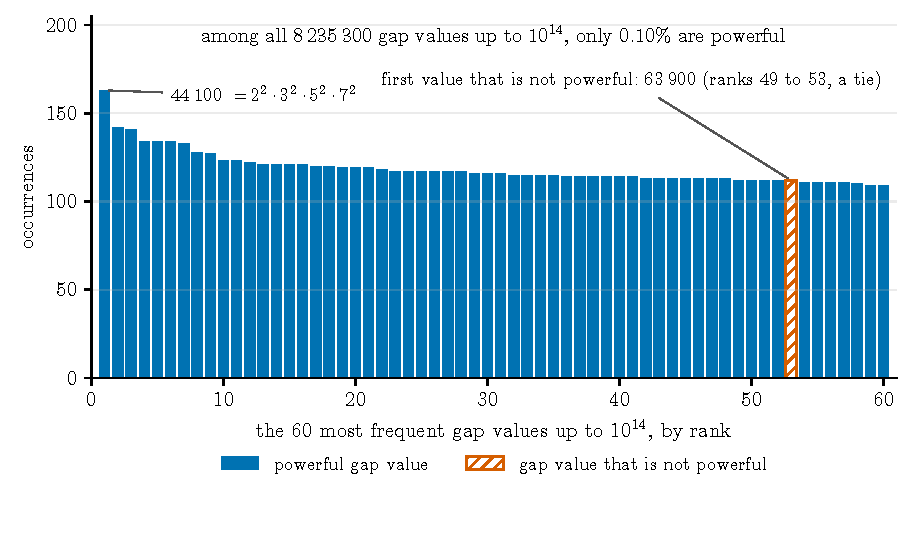
\includegraphics[width=\textwidth]{fig_luecken}
\caption{\textbf{Up to $10^{14}$, the \Z{lsbis} most frequent gap values are all powerful, although only \Z{lsanteil}\,\% of all gap values are.}
The sixty most frequent values of the gap between consecutive powerful numbers up to $10^{14}$, by their number of occurrences; values with
the same number share their rank and are ordered by size. The first \Z{lsbis} values are all powerful; the first
value that is not powerful, $\Z{lserster}$, shares its number of occurrences with powerful values (Proposition~\tref{prop:kopf}). Among all
\Z{lswerte} gap values up to $10^{14}$, only \Z{lsanteil}\,\% are powerful. The all-powerful head is shorter at $10^{14}$ than at $10^{12}$
(Table~\ref{tab:kopf}), so the picture says nothing about larger bounds (Question~\tref{q:luecken}).}\label{fig:luecken}
\end{figure}

\section{The gap spectrum of powerful numbers}\tlabel{sec:luecken}

Write the powerful numbers in increasing order and call the difference $g$ of two consecutive members a \emph{gap}; the sequence of gaps is
OEIS A076446 \cite{OEISA076446}. For an integer $g \ge 1$ let $\operatorname{sqfull}(g)$ be the product of the prime powers $p^{v_p(g)}$ with
$v_p(g) \ge 2$. Then $\operatorname{sqfull}(g) = g$ holds exactly when $g$ is powerful. Up to $10^{14}$ there are \Z{lsnpw} powerful numbers
and \Z{lswerte} distinct gap values, and only \Z{lsanteil}\,\% of these values are powerful; most of them are large and occur once. Among
the \Z{lsbasiswerte} values that occur at least \Z{lsbasismind} times, \Z{lsbasisanteil}\,\% are powerful. This section shows that the most
frequent gap values are nevertheless powerful, and gives a mechanism that favors them.

\begin{lemma}[Bajpai, Bennett and Chan {\cite[proof of Theorem~1.1]{BajpaiBennettChan2024}}]\tlabel{lem:ggt}\belegart{literature}
Let $n$ and $n + g$ be powerful. Then $\gcd(n, g)$ is powerful and divides $\operatorname{sqfull}(g)$. In particular $\gcd(n, g) = 1$ if $g$
is squarefree, and $g \mid n$ is possible only if $g$ is powerful.
\end{lemma}

\begin{proof}
If a prime $p$ divides $n$ and $g$, it divides $n + g$, so $p^2$ divides $n$ and $n + g$ and hence their difference $g$. So every prime of
$\gcd(n, g)$ occurs in it at least twice, and with an exponent at most $v_p(g)$, where $v_p(g) \ge 2$. If $g \mid n$, then
$\gcd(n, g) = g$ is powerful.
\end{proof}

That $\gcd(n, g)$ is powerful is used, for $k$-full numbers and without a separate proof, by Bajpai, Bennett and Chan immediately before
their equation~(4.2); the consequence for $\operatorname{sqfull}(g)$ is immediate, and it is what we use.

\inwords If two powerful numbers are a distance $g$ apart, every prime they share with $g$ appears in $g$ at least twice. So the part of
$g$ that such a pair can share is its powerful part; for a gap without square factors there is nothing to share.

\begin{proposition}[the head of the gap spectrum]\tlabel{prop:kopf}\belegart{computed}
Up to $10^{14}$ the \Z{lsbis} most frequent gap values are all powerful; they are the values that occur more than \Z{lsocc} times. The first
value that is not powerful is $\Z{lserster} = 2^2 \cdot 3^2 \cdot 5^2 \cdot 71$, with \Z{lsocc} occurrences, and it is the only one among
the \Z{lsg100} values that occur at least as often as the hundredth most frequent. Among the \Z{lsg200} values that occur at least as often as
the two hundredth, \Z{lsg200pw} are powerful. Table~\ref{tab:kopf} gives the same count at $10^{12}$ and $10^{13}$.
\end{proposition}

\begin{table}[ht]
\centering
\small
\setlength{\tabcolsep}{3pt}
\begin{tabular}{rrrrrrrr}
\hline
 & powerful & gap & \% of values & most & all powerful & first value & powerful near \\
bound & numbers & values & powerful & frequent & to rank & not powerful & rank $200$ \\
\hline
\Z{lstab}
\hline
\end{tabular}
\caption{The gap values between consecutive powerful numbers up to three bounds (Proposition~\tref{prop:kopf}). Values of equal frequency
share a rank; the column ``all powerful to rank'' counts the values that occur more often than the first value that is not powerful,
and the last column counts the powerful values among those that occur at least as often as the two hundredth most frequent.}
\label{tab:kopf}
\end{table}

If the $50$ most frequent values were drawn at random from all gap values up to $10^{14}$, about \Z{lserwartet} of them would be powerful,
and about \Z{lsbasiserw} if they were drawn from the values that occur at least \Z{lsbasismind} times.
The most frequent value at $10^{13}$ and $10^{14}$ is $\Z{lstop1} = 2^2 \cdot 3^2 \cdot 5^2 \cdot 7^2$.

\inwords Almost no gap value is powerful, but nearly all of the frequent ones are. From $10^{12}$ to $10^{14}$ the share of powerful values near
the top rises, while the first exception moves up the list; the effect does not simply grow or fade with the bound.

\begin{remark}[a ceiling for common divisors]\tlabel{rem:decke}\belegart{computed}
By Lemma~\tref{lem:ggt}, a pair at gap $g$ shares at most $\operatorname{sqfull}(g)$ with $g$, and only a powerful $g$ can share all of
itself. Table~\ref{tab:decke} lists the \Z{lsdeckeanz} values that are not powerful among the \Z{lsg200} values of
Proposition~\tref{prop:kopf}. Each has a small powerful part that is itself a frequent gap value; values of equal frequency share a rank, so
the rank is given as a range. The share of occurrences in which the pair shares the full ceiling is \Z{lsanteilpw}\,\% for the \Z{lsg20}
values that occur at least as often as the twentieth most frequent, and \Z{lsanteilnpw}\,\% for these \Z{lsdeckeanz}. So both sides are
consistent with one mechanism, a pair sharing the largest divisor that the lemma allows; only the size of that divisor differs.
\end{remark}

\begin{table}[ht]
\centering
\small
\begin{tabular}{rrrrr}
\hline
$g$ & $\operatorname{sqfull}(g)$ & rank of $\operatorname{sqfull}(g)$ & occurrences of $g$ & \% with $\gcd = \operatorname{sqfull}(g)$ \\
\hline
\Z{lsdecke}
\hline
\end{tabular}
\caption{The frequent gap values up to $10^{14}$ that are not powerful (Remark~\tref{rem:decke}): all values that are not powerful and
occur at least as often as the two hundredth most frequent.}\label{tab:decke}
\end{table}

\inwords About half of the pairs at gap $\Z{lserster}$ share the factor $900$ with the gap, and $\Z{lserster}$ occurs nearly as often as
$900$ itself. A powerful gap can share all of itself with a pair; this is one reason why the head of the spectrum is powerful, not a proof
that it must be.

\begin{remark}[a counting model, measured]\tlabel{rem:zaehlmodell}\belegart{measured}
Write $g = \operatorname{sqfull}(g) \cdot c$ with $c$ squarefree, and let $\operatorname{occ}(g)$ be the number of occurrences of $g$ up to
$10^{14}$. Over the \Z{zmn} gap values with at least \Z{zmmin} occurrences, which have \Z{zmkerne} distinct parts $\operatorname{sqfull}(g)$
and \Z{zmkof_n} distinct cofactors $c$, we fitted $\log \operatorname{occ}(g) = u(\operatorname{sqfull}(g)) + v(c)$ with one free value per
part and per cofactor. Evaluated on the values held back from the fit, in five random splits of about four fifths to one fifth over the gap
values, with the mean effect used for a part or cofactor that the fit has not seen and an affine recalibration fitted on the training part,
the model accounts for $\Z{zmr2} \pm \Z{zmr2sd}$ of the variance of $\operatorname{occ}(g)$ and $\Z{zmr2log} \pm \Z{zmr2logsd}$ of the
variance of $\log \operatorname{occ}(g)$, against $\Z{zmroh} \pm \Z{zmrohsd}$ for a regression of $\operatorname{occ}(g)$ on plain arithmetic
features of $g$ on the same values; the margin is positive in each split. The part alone accounts for \Z{zmkern}, the cofactor alone for
\Z{zmkof}, and on the fitted values the product $u \cdot v$ is uncorrelated with the residuals ($r = \Z{zmww}$). The values of $v$ are
reproducible up to a reliability of \Z{zmdecke}, which bounds what any explanation of $v$ can reach; on the \Z{zmdeutstufen} cofactors with
at least \Z{zmdeutkmin} gap values, the size and the prime factors of $c$ account for \Z{zmdeutung} of $v$ on held-back cofactors in one
split, against a ceiling of \Z{zmdeutdecke} measured on the same cofactors.
\end{remark}

The lemma therefore explains why the most frequent values can be powerful, not how often a value occurs: in this model the powerful part
alone accounts for \Z{zmkern} of the variance and the squarefree rest for \Z{zmkof}. This is a measurement on a finite range and not a
statement about all gaps. A version that splits $g$ over all its powerful divisors
instead of the canonical one fits the counts of the observed pairs $(g, \gcd)$ closely, but does not predict new gap values significantly better than the plain
arithmetic features ($\Z{zmallesep} \pm \Z{zmallesepsd}$ against $\Z{zmalleroh} \pm \Z{zmallerohsd}$), because about half of its cofactors
occur at a single gap; the record of this negative result is part of the deposit.

\inwords For the gap values that occur at least \Z{zmmin} times, knowing the powerful part and the squarefree rest of a gap predicts about half
of the variation in how often it occurs, and the rest matters more than the powerful part. The prediction was tested on gaps that the fit
had not seen. It describes the data up to $10^{14}$; it is not a law.

\begin{remark}[common factors of pairs]\tlabel{rem:primitiv}\belegart{measured}
In a sample of every \Z{pmschritt}th consecutive pair up to $10^{14}$, \Z{pmstich} pairs in total, the two members are coprime in
\Z{pmanteil}\,\% of the cases. The most frequent common divisors are \Z{pmgcd}, all powerful, as Lemma~\tref{lem:ggt} requires.
\end{remark}

\inwords About half of the neighboring pairs of powerful numbers share a factor, and the shared factor is always powerful.

We also computed the number variance of the powerful numbers in windows of up to \Z{nvlmax} mean spacings. It lies within about
\Z{nvrel}\,\% of a sum of independent lattice variances, and the large-window form of that sum grows like $L^{2/3}$ with the constant of
Chan's theorem \cite[Theorem~2]{Chan2026Variance}; in our windows the measured growth, a slope of \Z{nvsteig} on a logarithmic scale, has not
yet reached the exponent $2/3$. This is a check of Chan's theorem and not a new result.

\emph{Prior art and its reach.} Apart from the lemma, we found no work on the distribution of the gap values between powerful numbers.
We checked the work of Bajpai, Bennett and Chan in full, the OEIS entries A076446 and A001694, and records on Zenodo; the citing works of
Bajpai, Bennett and Chan were queried in two databases, which returned three and none. The reach of this search is set by these databases.

\section{Powerful values of cyclotomic polynomials}\tlabel{sec:zyklotomisch}

Remark~\partref{I}{rem:zyklotomisch} explains where these values come from. If a member of a triple is a proper power $x^r$ with $r \ge 2$,
its neighbors $x^r - 1$ and $x^r + 1$ are products of values $\Kreis{e}(x)$ and $\Kreis{e}(-x)$ of cyclotomic polynomials. Two such values
share only primes that divide $2r$, so a value that is coprime to the others must itself be powerful. This section records what we know
about powerful values $\Kreis{d}(x)$ at integers $x \ge 2$. For $d = 3$, $4$ and $6$ the polynomial is quadratic, and the question belongs to
the study of powerful values of quadratic polynomials by De Koninck, Doyon and Luca \cite{DeKoninckDoyonLuca2011}.

\begin{remark}[the values $x^2 + 1$]\tlabel{rem:xquadrat}\belegart{computed}
A powerful number that is not a square can be written as $a^2 b^3$ with $b > 1$ squarefree, so $x^2 + 1 = \Kreis{4}(x)$ is powerful exactly
when $x^2 - b^3 y^2 = -1$ has a solution for some squarefree $b > 1$; this is the form (1)--(2) of De Koninck, Doyon and Luca
\cite[p.~2]{DeKoninckDoyonLuca2011}, and their Table~1 gives the smallest case, $682^2 + 1 = 5^3 \cdot 61^2$ \cite[p.~8]{DeKoninckDoyonLuca2011}.
For each such $b$ the solutions form an infinite family, the odd powers of the smallest one. We solved the equation for all \Z{znaqg}
squarefree $b$ with $1 < b \le \Z{znab}$: it has a solution for \Z{znamit} of them. The list of OEIS A175155 \cite{OEISA175155} of the values
$x$ with $x^2 + 1 = a^2 b^3$ begins $682$, $1\,268\,860\,318$, $1\,459\,639\,851\,109\,444$.
\end{remark}

\inwords The number $x^2 + 1$ is powerful for infinitely many $x$, but such $x$ are very sparse: after $682$ the next value in the
list of OEIS A175155 is above a billion. Each of them comes from a Pell-type equation, and only some of these equations have solutions.

\begin{proposition}[two explicit chains of powerful values of $\Kreis{3}$ and $\Kreis{6}$]\tlabel{prop:phidrei}\belegart{proved}
Let the map $(y, m) \mapsto (127 y + 672 m,\ 24 y + 127 m)$ act on the starting points $(37, 7)$ (the first chain) and $(5, 1)$ (the
second chain), and let $(y_j, m_j)$ be the point after $j$ steps. In both chains $y_j^2 - 28 m_j^2 = -3$ and $y_j$ is odd for every $j$; $7 \mid m_j$ exactly when
$j \equiv 0 \pmod 7$ in the first chain and exactly when $j \equiv 6 \pmod 7$ in the second; and the two chains contain every solution of
$y^2 - 28 m^2 = -3$ with $y, m > 0$. For every $j$ with $7 \mid m_j$ the number $x = (y_j - 1)/2$ satisfies
$\Kreis{3}(x) = 343\,(m_j/7)^2$, which is powerful, and $\Kreis{6}(x + 1) = \Kreis{3}(x)$. In particular $\Kreis{3}(x)$ and $\Kreis{6}(x)$ are
powerful for infinitely many $x$.
\end{proposition}

\begin{proof}
Since $127^2 - 28 \cdot 24^2 = 1$, the map preserves $y^2 - 28m^2$, and $37^2 - 28 \cdot 7^2 = 5^2 - 28 \cdot 1^2 = -3$. It preserves the parity
of $y$, because $672$ is even and $127$ is odd. Modulo $7$ it fixes $y$, because $672 \equiv 0$ and $127 \equiv 1$, and it adds $24 y \equiv 3y$ to
$m$. In the first chain $y_0 \equiv 2$ and $m_0 \equiv 0 \pmod 7$, so $m_j \equiv 6j \pmod 7$, which vanishes exactly when $j \equiv 0 \pmod 7$; in
the second $y_0 \equiv 5$ and $m_0 = 1$, so $m_j \equiv 1 + 15j \equiv 1 + j \pmod 7$, which vanishes exactly when $j \equiv 6 \pmod 7$.
For the completeness, let $\alpha = y + z\sqrt 7$ with $y, z > 0$ and $y^2 - 7z^2 = -3$. Its conjugate is $-3/\alpha$, so $2y = \alpha - 3/\alpha > 0$
gives $\alpha > \sqrt 3$. Dividing by $\varepsilon = 8 + 3\sqrt 7$ keeps the norm, and keeps the quotient above $\sqrt 3$ as long as $\alpha > \sqrt 3\,\varepsilon$;
so $\alpha = \beta \varepsilon^n$ with $n \ge 0$ and $\sqrt 3 < \beta \le \sqrt 3\,\varepsilon$. For $\beta = y' + z'\sqrt 7$ this gives
$z' = (\beta + 3/\beta)/(2\sqrt 7) < \sqrt 3\,(\varepsilon + 1)/(2\sqrt 7) < 6$, and among $1 \le z' \le 5$ only $z' = 1$ and $z' = 2$ make $7z'^2 - 3$ a
square, so $\beta = 2 + \sqrt 7$ or $\beta = 5 + 2\sqrt 7$. Multiplying by $\varepsilon$ replaces $(y, z)$ by $(8y + 21z, 3y + 8z)$, which swaps the
parities of $y$ and $z$; so $z = 2m$ is even exactly for $(2 + \sqrt 7)\varepsilon^n$ with $n$ odd and for $(5 + 2\sqrt 7)\varepsilon^n$ with $n$ even. Since
$(2 + \sqrt 7)\varepsilon = 37 + 14\sqrt 7$ and $\varepsilon^2 = 127 + 48\sqrt 7$, these are the two chains, and multiplying by $\varepsilon^2$ is the map. Finally
$4\Kreis{3}(x) = (2x + 1)^2 + 3 = y_j^2 + 3 = 28 m_j^2$, so $\Kreis{3}(x) = 7 m_j^2$, and $\Kreis{6}(x + 1) = (x + 1)^2 - (x + 1) + 1 =
\Kreis{3}(x)$.
\end{proof}

In the first chain the first member is $x = 18$ with $\Kreis{3}(18) = 7^3$; the next three have \Z{phidreistellen} digits. The value $x = 18$ is the entry
$k = 3$, $n = 37$ of Table~1 of De Koninck, Doyon and Luca, since $37^2 + 3 = 4\,\Kreis{3}(18)$ \cite[p.~8]{DeKoninckDoyonLuca2011}, and
they observe that for a quadratic polynomial one powerful value of this kind gives infinitely many \cite[p.~7]{DeKoninckDoyonLuca2011}.
Their reduction on that page, applied to $\Kreis{3}$ with squarefree part $7$, leads in our normalization to the equation
$y^2 - 28m^2 = -3$ with $7 \mid m$. We did not find there the explicit recurrence, the two chains and their completeness, the parity of
$y_j$, the period $7$, or the transfer to $\Kreis{6}$. A direct search over all $m \le \Z{phidreibrute}$ finds no solution outside the two
chains, as the proposition says. The two chains are
disjoint: going forward from $(5, 1)$ the values of $y$ are $5, 1307, \dots$, going backward they are negative from $(-37, 7)$ on, so $(37, 7)$
is not on the second chain. The prime $x$ with $\Kreis{3}(x) = 7^3 a^2$ reported by Lavi \cite{Lavi2026}, which we know from the description of his record, is the
member $j = \Z{phidreilavij}$ of the second chain. Other squarefree parts give other powerful values: the second value for $d = 3$ in
Table~\ref{tab:zyk} comes from the equation $y^2 - 52 m^2 = -3$ with $13 \mid m$, that is, with $13$ in place of $7$.

\inwords The polynomials $x^2 + x + 1$ and $x^2 - x + 1$ take powerful values infinitely often. A Pell equation produces them one after
another, in two chains, and every seventh step of each chain gives one. The idea that one solution gives infinitely many is in the
literature; we did not find the explicit chains there.

\begin{proposition}[powerful values up to a bound]\tlabel{prop:zyktafel}\belegart{computed}
Among the \Z{zykn} pairs $(d, x)$ with $3 \le d \le 12$, $x \ge 2$ and $\Kreis{d}(x) \le \Z{zykschranke}$, exactly \Z{zyktreffer} give a
powerful value $\Kreis{d}(x)$. They are listed in Table~\ref{tab:zyk}.
\end{proposition}

\begin{table}[ht]
\centering
\small
\begin{tabular}{rrrl}
\hline
$d$ & $x$ & $\Kreis{d}(x)$ & factorization \\
\hline
\Z{zyktab}
\hline
\end{tabular}
\caption{The powerful values $\Kreis{d}(x)$ with $3 \le d \le 12$ and $\Kreis{d}(x) \le \Z{zykschranke}$ (Proposition~\tref{prop:zyktafel}).
The pairs for $d = 3$ and $d = 6$ are related by $\Kreis{6}(x + 1) = \Kreis{3}(x)$.}\label{tab:zyk}
\end{table}

\inwords Up to the bound, powerful cyclotomic values occur only for $d = 3, 4, 5$ and $6$, and only \Z{zyktreffer} times. The case $d = 5$ is
$3^4 + 3^3 + 3^2 + 3 + 1 = 121 = 11^2$, a square.

\begin{remark}[a class without squares]\tlabel{rem:granvilleklasse}\belegart{computed}
The numbers $x_n = (x^n - 1)/(x - 1)$ satisfy $x_{n+2} = (x + 1)\,x_{n+1} - x\,x_n$, a recurrence with $b = x + 1$ and $c = -x$ coprime and
$b^2 + 4c = (x - 1)^2 > 0$. If $x \equiv 2 \pmod 4$, then $c \equiv 2 \pmod 4$, and Granville's theorem \cite[Theorem~3]{Granville2012} gives, for every
$d \notin \{1, 2, 3, 6\}$, a primitive prime factor of $x_d$ that divides it to an odd power. Such a prime divides $\Kreis{d}(x)$ and no
$\Kreis{e}(x)$ with $e \mid d$, $e < d$, so $\Kreis{d}(x)$ is not a square. It can still be powerful, since an odd exponent can be $3$. We
checked the consequence: for $x \equiv 2 \pmod 4$, $d \in \{4, 5, 7, \dots, 12\}$ and $\Kreis{d}(x) \le \Z{zykklasse}$ no value is a
square, while outside the class the square $\Kreis{5}(3) = 11^2$ appears at once, and for these degrees it is the only square outside the
class up to $\Z{zykklasse}$. Inside the class, $\Kreis{4}(682) = 5^3 \cdot 61^2$ is powerful without being a square.
\end{remark}

\inwords For arguments of the form $4j + 2$, a theorem of Granville shows that the cyclotomic values are never squares, apart from four
small degrees. Our check up to $\Z{zykklasse}$ agrees with it, and the example $\Kreis{5}(3) = 121$ shows that the condition on the argument cannot simply be
dropped. The theorem says nothing about cubes, so it does not decide whether such a value can be powerful.

\begin{proposition}[the simplest case of $\Kreis{8}$]\tlabel{prop:phiacht}\belegart{proved}
There are no positive integers $x$ and $a$ and no prime $q < 2 \cdot 10^{11}$ with $x^4 + 1 = q^3 a^2$.
\end{proposition}

\begin{proof}
For $q = 2$ there is nothing to prove, since $x^4 + 1 \equiv 1$ or $2 \pmod{16}$ while $8a^2 \equiv 0$ or $8 \pmod{16}$. Let $q$ be odd and
write $x^4 + 1 = q\,y^2$ with $y = qa$. By Cohn \cite[p.~1347 and Theorem~1]{Cohn1997b}, a solution requires $q \equiv 1 \pmod 8$ and a
solution of $v^2 - q u^2 = -1$; if $\alpha = c + b\sqrt{q}$ is the smallest one, $u_n = (\alpha^n - \bar\alpha^n)/(2\sqrt q)$ and
$v_n = (\alpha^n + \bar\alpha^n)/2$, then $x^2 = v_A$ and $y = u_A$, where $A$ is the squarefree part of $c$. Expanding $\alpha^n$ gives $u_n \equiv n\,c^{n-1} b \pmod q$. Since
$c^2 \equiv -1 \pmod q$, the prime $q$ divides neither $c$ nor $A$, so $q \mid y = u_A$ forces $q \mid b$. For $q \equiv 1 \pmod 8$ the
fundamental unit $(t + w\sqrt q)/2$ of $\mathbb{Q}(\sqrt q)$ has $t$ and $w$ even, because $t^2 - q w^2 = \pm 4$ is impossible with $t$
and $w$ odd; so it lies in $\mathbb{Z}[\sqrt q]$, equals $\alpha$, and $b = w/2$. Hence a solution requires $q \mid w$. The conjecture of
Ankeny, Artin and Chowla says that this never happens, and it has been verified for all primes $q \equiv 1 \pmod 4$ below $10^{11}$
\cite{vanderPoortenteRieleWilliams2001} and between $10^{11}$ and $2 \cdot 10^{11}$ \cite{vanderPoortenteRieleWilliams2003}.
\end{proof}

We checked the last step independently for the \Z{achtq} primes $q \equiv 1 \pmod 8$ below $\Z{achtgrenze}$: in none of them does $q$
divide $b$. The proposition covers only the case in which the squarefree part of $x^4 + 1$ is a single prime. For small squarefree parts
the literature settles the question completely: Cohn solved $x^4 + 1 = D y^2$ for all squarefree $D < 10^5$, and apart from $D = x^4 + 1$
with $y = 1$ the only solution is $261^4 + 1 = 70\,258 \cdot 257^2$ \cite[abstract]{Cohn1997b}. If $x^4 + 1$ is powerful and $D$ is its
squarefree part, then $D \mid y$; neither case allows this, so the squarefree part of a powerful $x^4 + 1$ is at least $10^5$.

\inwords The number $x^4 + 1$ is the eighth cyclotomic value. If it were a cube of a prime times a square, a theorem of Cohn would force a
very special divisibility in the smallest solution of a Pell equation, and that divisibility is exactly what a well-tested conjecture
forbids; computer searches by others confirm it far enough to exclude all primes below $2 \cdot 10^{11}$.

\section{An independence test along the divisors of the index}\tlabel{sec:unabhaengig}

The heuristic of Part~I treats the event that a prime of rank $d$ divides $T_d(m)$ at least twice as a rare event of probability about
$1/p$, independent of other such events (Proposition~\partref{I}{prop:exponenten}). Part~I tests independence across the primes of one
kernel. A lattice point $(m, k)$ with many divisors carries one such event for each divisor $d$ of $k$, and the divisors are linked: $q d$ is
a multiple of $d$. This section tests whether the events at $d$ and at $q d$ are coupled.

\begin{remark}[no joint event along the divisors, and the power of the test]\tlabel{rem:unabhaengig}\belegart{measured}
For the \Z{ukerne} kernels with the most lattice points in the box of Theorem~\partref{I}{thm:reduktion}, we took each rank $d$ and its smallest prime $p$ of rank $d$ below $\Z{up}$, and set
the status of $d$ to $1$ if $p^2 \mid T_d(m)$ and to $0$ otherwise. We then formed all pairs $(d, qd)$ with $q \in \{3, 5, 7, 11, 13\}$ for
which both ranks have such a prime: \Z{upaare} pairs. The status is $1$ at $d$ alone in \Z{u10} pairs, at $qd$ alone in \Z{u01}, and at both
in \Z{u11}; independence predicts \Z{uerw} pairs with both. To see what this test could detect, we simulated a coupling in which the status
at $qd$ copies the status at $d$ with probability $\rho$, independently for each pair: for $\rho = 0.1$ one expects about \Z{ukopie} copied
pairs, and in at least \Z{utrenn}\,\% of \Z{usim} simulations at least one joint event appeared, against less than \Z{utrennnull}\,\% for
$\rho = 0$.
\end{remark}

\inwords If the rare event at one rank made the same event at a multiple rank more likely, pairs with the event at both ranks would appear.
There are none. The test is not blind: a coupling in which one time in ten the second event copies the first would almost always have shown
up, and one of half that strength would still have shown up in most runs. A much weaker coupling, or one that makes the second event less
likely, could not be seen with so few events, and the test uses only the smallest prime of each rank.

The test is formally a $\chi^2$ test on the table, but with fewer than one expected joint event the statistic only records whether a joint
event occurs; the simulation measures exactly that. One event at a rank $d$ enters a pair for each $q$ with $qd$ occupied, so the \Z{u10}
pairs come from fewer distinct events; the simulation copies pair by pair and therefore overstates the power against a coupling that acts
once per event. In the prior-art search for this part (arXiv, Zenodo, Google Scholar and OEIS, at the level of titles and abstracts) we found
no earlier test of independence along the divisors of the index.

\section{Wieferich fractions of Pell units}\tlabel{sec:linsen}

For a squarefree $m$ and a prime $p \nmid 2m$ let $e = \left(\frac{m}{p}\right)$ and write $\varepsilon_m^{\,p - e} = A + B\sqrt m$ modulo $p^2$.
Then $A \equiv 1$ and $B \equiv 0 \pmod p$, and we call $y_p = \bigl((B/p) \bmod p\bigr)/p \in [0, 1)$ the \emph{Wieferich fraction} of
$\varepsilon_m$ at $p$. It vanishes exactly when the order of $\varepsilon_m$ modulo $p^2$ equals its order modulo $p$; for a prime with a
rank this is the condition $p^2 \mid T_{\alpha_m(p)}(m)$ of Part~I. In Katz's language \cite{Katz2015}, $\varepsilon_m$ is a point on the torus
$x^2 - m y^2 = 1$, and $y_p$ is its Wieferich fraction for the framing whose Lie lattice is $\mathbb{Z}\sqrt m$, which Katz describes
\cite[Section~6]{Katz2015}. His Framed Wieferich Conjecture \cite[Conjecture~6.1]{Katz2015} predicts that such fractions are equidistributed.

\begin{remark}[no deviation from equidistribution, memory or coupling]\tlabel{rem:wieferichbrueche}\belegart{measured}
For the \Z{wf3kerne} kernels of Section~\tref{sec:unabhaengig} and all primes $p < \Z{wf3p}$ with $p \nmid 2mU_1$, that is, for \Z{wfn} pairs
$(m, p)$, we computed $y_p$.
\begin{enumerate}
\item[(a)] \emph{Near zero.} For six thresholds $t$ from $10^{-2}$ to $10^{-7}$ the number of $y_p < t$ agrees with the exact expectation for
  uniform $y_p$; the largest deviation is $\Z{wfzmax}$ standard deviations. For example, $y_p < 10^{-4}$ holds \Z{wft4b} times against
  \Z{wft4e} expected, and $y_p = 0$ holds \Z{wftreffer} times against $\sum 1/p = \Z{wferw}$. Only \Z{wfnullrang} of these zeros lie at primes that divide
  some $T_k(m)$, which happens exactly when the order of $\varepsilon_m$ modulo $p$ is divisible by $4$; they are the Wieferich events of
  Part~I on these kernels (Remark~\partref{I}{rem:wfdaten}), and the other zeros do not appear there. Split by the $2$-adic valuation of the order of
  $\varepsilon_m$ modulo $p$ (odd, $2 \bmod 4$, $0 \bmod 4$) and by $e$ into \Z{wfklanz} classes, the smallest $p$-value of a $\chi^2$ test
  of uniformity is \Z{wfklpmin}, or \Z{wfklbon} after the Bonferroni correction.
\item[(b)] \emph{Along the primes.} For each kernel, the correlation of $y_p$ with the fraction $j$ primes later, for $j = 1, \dots,
  \Z{wglags}$, gives \Z{wgtests} tests; \Z{wgueber} exceed $|z| = 2.576$ against about \Z{wgerw} expected, the largest is $\Z{wgzmax}$, with
  Bonferroni $p = \Z{wgpbon}$. A memory planted in test data, with $5$ percent of the values replaced by their predecessor, is found with
  $z = \Z{wgpk}$.
\item[(c)] \emph{Between kernels.} For the \Z{wkpaare} pairs of kernels, the correlation of their fractions at common primes has largest
  $|z| = \Z{wkzmax}$, with Bonferroni $p = \Z{wkpbon}$; a planted correlation of strength $0.02$ is found with $z = \Z{wkpk}$.
\end{enumerate}
\end{remark}

\inwords For every unit and every prime there is a number between $0$ and $1$ that measures how close the prime comes to being a
Wieferich prime for that unit. Over more than five million such numbers, on \Z{wf3kerne} units and the primes below $\Z{wf3p}$, our tests find no deviation from independent uniform random numbers: near zero,
from one prime to the next, and from one unit to another. Katz's conjecture predicts (a); applied to the product of two such tori it also
predicts (c); (b) goes beyond it. The only computation of Wieferich fractions that his paper mentions is one for elliptic curves, by
Bombieri, reported as compatible with the conjecture. Censuses of the zeros $y_p = 0$ exist for single units, for example Ryan's for
$1 + \sqrt 2$ up to $10^9$ \cite[Sections~2.1 and~5.1]{Ryan2026}; we did not find a test of the distribution of the fractions themselves,
near zero, along the primes or between units. A finite test cannot prove equidistribution; it shows no deviation at the sizes the controls
can detect.

\section{Questions}\tlabel{sec:fragen}

\begin{question}[the most frequent gap]\tlabel{q:luecken}\belegart{open}
Let $g(x)$ be the most frequent gap between consecutive powerful numbers up to $x$. Is $g(x)$ powerful for all large $x$, and does the share
of powerful values among the $N$ most frequent gaps up to $x$ tend to $1$ when $N$ is fixed and $x \to \infty$?
\end{question}

Proposition~\tref{prop:kopf} and Table~\ref{tab:kopf} are consistent with the first part at three bounds up to $10^{14}$. For the second
part they point both ways: the share of powerful values among the two hundred most frequent rises, while the leading block in which all
values are powerful shrinks. Lemma~\tref{lem:ggt} gives powerful gaps an advantage; it does not show that the advantage wins in the limit.

\inwords Is the most common distance between neighboring powerful numbers always itself powerful, however far one looks? Up to $10^{14}$ it
is, but the data do not show a clear trend for the values just below the top.

\begin{question}[powerful values of $x^4 + 1$]\tlabel{q:phiacht}\belegart{open}
Is $x^4 + 1$ powerful for some integer $x \ge 1$?
\end{question}

By Proposition~\tref{prop:phiacht} and the paragraph after it, the squarefree part of such a value is at least $10^5$, and it is not a prime
below $2 \cdot 10^{11}$. For $x^2 + 1$ the answer is yes (Remark~\tref{rem:xquadrat}).

\inwords Can the eighth cyclotomic value $x^4 + 1$ ever be powerful? The fourth one, $x^2 + 1$, can. For $x^4 + 1$ only special shapes are
excluded so far.

\begin{remark}[a conjecture on the most frequent gap]\tlabel{rem:champion}\belegart{heuristic}
We state a weak and a strong form for the most frequent gap $g(x)$ of Question~\tref{q:luecken}. \emph{Weak form:} $g(x)$ tends to infinity with $x$,
and $g(x)$ is powerful for all large $x$. \emph{Strong form:} for all large $x$, $g(x)$ is the square of a product of the first primes,
$(2 \cdot 3 \cdots p_r)^2$, with $r$ growing with $x$. The strong form implies the weak one; the weak one claims only what the data and
Lemma~\tref{lem:ggt} support directly, and the strong one also names the shape. Up to $10^{12}$ the most frequent value
is $900 = (2 \cdot 3 \cdot 5)^2$, and up to $10^{13}$ and $10^{14}$ it is $\Z{lstop1} = (2 \cdot 3 \cdot 5 \cdot 7)^2$ (Table~\ref{tab:kopf}).
The reason we expect it is Lemma~\tref{lem:ggt}: if $g = P^2$ with $P$ squarefree and $P^2 \mid n$, then $n = P^2 m$ and
$n + g = P^2 (m + 1)$, so the primes of $P$ already occur at least twice in both numbers, and only the other primes of $m$ and $m + 1$
must occur squared. A larger $P$ frees more primes but leaves fewer $m \le x/P^2$; the smallest primes free the most for the smallest
cost, and as $x$ grows the balance moves to a larger $P$. A balance of this kind is behind the conjecture of Odlyzko, Rubinstein and Wolf
that the most frequent gap between consecutive primes eventually runs through the products of the first primes, $30$, $210$, $2310$
\cite{OdlyzkoRubinsteinWolf1999}; we found no such statement for powerful numbers. Two values do not make a trend. The weak form fails if
$g(x)$ stays bounded, or if a value that is not powerful is the most frequent gap for arbitrarily large $x$. The strong form fails in
addition if a powerful value of another shape, such as $3600$ or $3528$, which follow $900$ and $44\,100$ closely in the counts, is the most
frequent gap for arbitrarily large $x$. Which of the two forms is right is open.
\end{remark}

\inwords We expect the most common distance between neighboring powerful numbers to keep growing and to stay powerful (weak form), and
we suspect that it is always the square of $2 \cdot 3 \cdot 5 \cdots$, as $900$ and $44\,100$ are (strong form). For the primes a similar pattern is conjectured, with $30$, $210$, $2310$. This
is an expectation supported by two values and a mechanism, not a result.

\section*{The type of every statement}

Every statement of this part carries one of six labels, printed after its number. The table lists them; it is generated from the
text by the build and checked against a second, independent reading of the source.

\input{../gemeinsam/belegtab_\teilnr}

%
%
%
%
%
\section*{Data and code availability}\addcontentsline{toc}{section}{Data and code availability}

Every number of this \ifimband volume\else part\fi\ that we computed is generated from a result file of a data deposit or from a cited constant; no computed number is
typed by hand. The data deposit is archived with the collected volume, DOI \href{https://doi.org/10.5281/zenodo.23127547}{10.5281/zenodo.23127547}.

\paragraph{What the deposit contains.} The deposit has two parts. The core holds what the text cites: (i) the result files, in JSON and
plain text, behind every computed number, together with the raw output of the scripts that wrote them; (ii) the scripts, written in Python,
each stating before it runs what it expects to find and the positive and negative controls that it runs; (iii) a manifest with the SHA-256 hash
and the size of every file, which the build checks before it reads a result file; (iv) the decimal expansions of the building blocks of
Part~I that the searches left open (Proposition~\partref{I}{prop:raenge}), including those that the algebraic split of
Remark~\partref{I}{rem:zweiprimitive} settles; (v) the certificates and the second routes for the computations that settle a building block; and
(vi) the file \texttt{OPEN\_PROBLEMS.md}, which lists the open problems of the volume. The archive holds the remaining scripts and results of the
investigation, including negative results that the text does not print.

\paragraph{Where the files are.} The collected volume and its three parts are published as four linked records on Zenodo, and the same files
are in one repository on GitHub. The record of the collected volume (DOI \href{https://doi.org/10.5281/zenodo.23127547}{10.5281/zenodo.23127547}) holds the volume and the whole deposit,
the core and the archive described above. The record of each part holds that part and the result files that its text cites, and links to the
record of the volume. The repository (\href{https://github.com/berkay-yueksel-sayim/erdos-364-365-powerful-numbers-pell}{github.com/berkay-yueksel-sayim/erdos-364-365-powerful-numbers-pell}) holds the four PDFs and the deposit, and its README lists the four records. The records of Parts~I, II and~III have the DOIs \href{https://doi.org/10.5281/zenodo.23127703}{10.5281/zenodo.23127703}, \href{https://doi.org/10.5281/zenodo.23127705}{10.5281/zenodo.23127705} and~\href{https://doi.org/10.5281/zenodo.23127707}{10.5281/zenodo.23127707}.

\paragraph{How the numbers get into the text.} The source of the text refers to each computed number by a key. A build tool reads the result
file named for the key, verifies it against the manifest, computes the number in its printed form, and writes it into the text; it stops if a key
has no source or if a file differs from the manifest. The same tool generates the table of the types of the statements and the list of open
problems from the source of the text, and it is part of the core.

\paragraph{Software.} The scripts use Python~3.12 with gmpy2~2.3, SymPy~1.14 and NumPy~2.4. The elliptic curve method and its relatives are run
with GMP-ECM~7.0.6 \cite{GMPECM706}, used as an installed program inside a container image built from the Debian package and not part of the
deposit; the recipe of the image is in the core. The elliptic curve certificates for primality were produced in the same way with
PARI/GP~2.17.2 \cite{PARI2172} and are part of the deposit; a separate program of ours checks each of them, so the result does not
depend on that program. Further work is planned to support these certificates with a second prover written independently by us. The
text is set with pdf\TeX.

\paragraph{Licenses.} The text and the data are licensed under the Creative Commons Attribution 4.0 International License (CC BY 4.0), and
the code under the Apache License, Version 2.0. Programs of others that the scripts use as tools, such as GMP-ECM, are not part of the
deposit and keep their own licenses.

%
%
%
%
%
%
%
%
%
\section*{Use of AI tools}\addcontentsline{toc}{section}{Use of AI tools}

Generative AI tools were used throughout this work: large language models of the Claude family by Anthropic, mainly Claude Opus~5 and~5.5,
and also Claude Fable~5.1 and Claude Sonnet~5.5 and~5, between August and October 2026,
through the Claude Code environment. They were used to draft the text and the mathematical arguments, to write the computer programs, to
run and check the computations, and to search for and read the literature. The author works independently, is not trained as a number
theorist, and learned the subject actively during the work; the tools made it possible to carry out and check computations on this scale. The author led the work in stages: each stage was
set by a prompt that stated what it should achieve, within a stage the tools followed a plan agreed with the author, and the author considered
the results before giving the next prompt, revising the plan when the results required it. The author contributed ideas where they helped and
framed how a problem should be attacked, decided which statements to keep, and is responsible for the content. The programs of the project,
including its own checking and build tools, were developed with the AI tools, and the author started the long computations, such as the
factor searches, on the author's own machine.

Several parts of the checking do not rest on these tools. The elliptic curve primality certificates were produced by PARI/GP~2.17.2 and are
verified by a separate program, and the factor searches use GMP-ECM~7.0.6. Every computed number is generated by a program from deposited
data or from a cited constant, and the programs carry positive and negative controls. Proofs, numbers and citations were also checked in
independent passes by further instances of the AI tools that were given no access to the drafting context. These tools are not authors.

\bibliographystyle{amsplain}
\bibliography{../gemeinsam/literatur}
\end{document}
